\documentclass[../main.tex]{subfiles}
\graphicspath{{\subfix{../../images/}}}

\begin{document}

\subsection{NICs}

NICs, or network interface cards is a device a computer \textbf{requires} for it to access networks.

\begin{figure}[H]
    \centering
    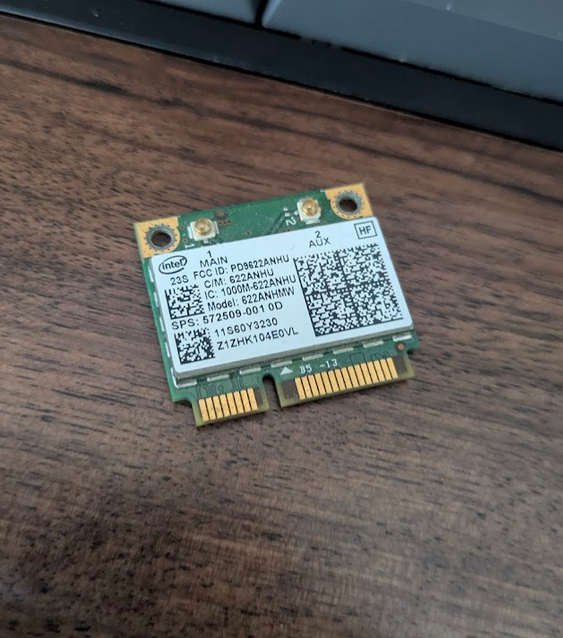
\includegraphics[width=0.7\textwidth]{nic.png}
    \caption{A network interface card used in a laptop.}
    \label{fig:nic}
\end{figure}

Specifically, this is a Wireless NIC, which allows it to connect to wireless (WiFi) networks. There are also standard NICs, which allows a computer to connect to wired networks.

\begin{itemize}
    \item NIC's are assigned \textbf{MAC addresses} from the manufacturer. See section \ref{2:sec:mac} for an in-depth explanation.
    \item When they connect to a network, they are assigned an \textbf{IP address} by the router. See section \ref{2:sec:ip} for an in-depth explanation.

\end{itemize}

\subsection{Routers}
\label{3:sec:routers}

A router allows data packets\footnote{For more information on packets, see \ref{2:sec:packet_switching} for details} to be transmitted between devices within a network, or outside a network. They typically have an internet cable plugged into it, and several cables going from the router to devices like a computer or other devices on the network.

\begin{figure}[H]
    \centering
    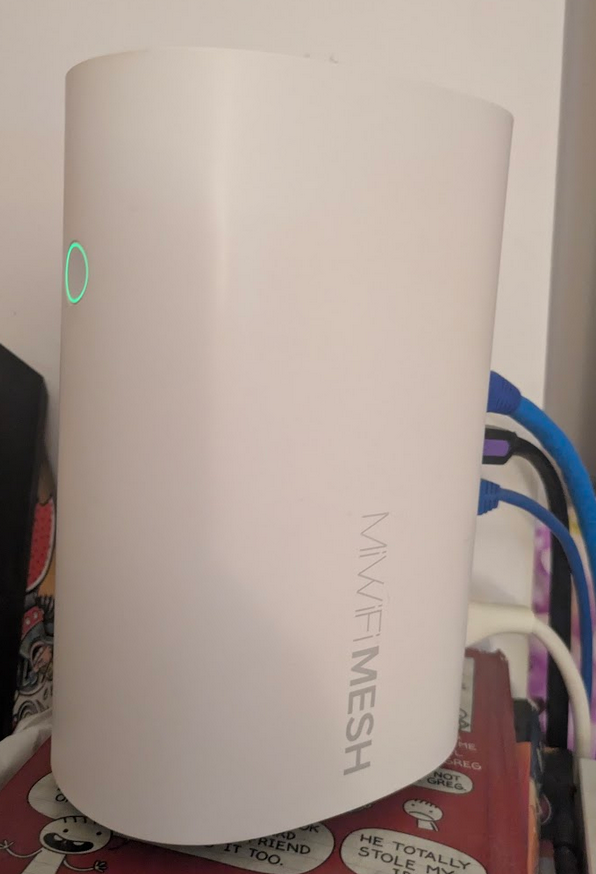
\includegraphics[width=0.5\textwidth]{router.png}
    \caption{A MiWiFi mesh router.}
    \label{fig:router}
\end{figure}

They play an \emph{essential role} in packet switching, as they are the devices that relays data packets around a wide area network (like all the homes in Singapore). So yes, \textbf{your router is relaying packets from your neighbor's home to your other neighbor's home!}

\end{document}
